\chapter{HBT-EP Capabilities}
\paragraph{}The HBT-EP Tokamak combines a highly configurable configuration with an extremely high resolution magnetic sensor set.  A close-fitting shell, consisting of 20 segments that cover 360$^{\circ}$ of toroidal angle and roughly 180$^{\circ}$ of poloidal angle (from bottom to top, along the outboard side) can be inserted or retracted to change the passive stabilization of the plasma.  On each of the shell segments are mounted two poloidally offset triplets of saddle coils which can be used to apply magnetic fields to the plasma surface for mode excitation or suppression.  Of each triplet, only one coil can be energized at a time, meaning that there are four toroidally complete rings of 10 coils each, in vessel, located less than 2cm from the nominal plasma surface.  Every coil in the system can be energized independently, with up to $\pm$ 40A of current.  This translates to \textbf{HOW MUCH} G at the nominal plasma surface from each coil.  \textbf{Should I include a Niko lot of field on surface?}  Detection of mode activity and response to feedback is accomplished by a set of 216 in-vessel sensors.  These sensors measure both radial and poloidal fields, and are arrayed in two complete poloidal rings, offset by 180 $^{\circ}$ of poloidal angle, one complete toroidal array on the inboard midplane, and four poloidally offset toroidal arrays on the outboard side.  Measurements provided by these sensors will be the basis for all analysis in this paper.
\section{The Plasma}
\subsection{Equlibrium Fields}
\subsubsection{Toroidal Field}
The Toroidal field is created by 20 coil packs connected in series.  The field on the nominal plasma axis is 3.3kG.  Due to the geometry of the currents that create the field, the magnitude of the field has a $\frac{1}{R}$ dependence.  Due to the discrete nature of the currents that create the field, there is a 'TF ripple' that modulates the toroidal field strength by textbf{WHAT}$\%$
\subsubsection{Ohmic Heating}
A solenoid passes through the center of the torus, and is connected to three capacitive power supplies.  They provide first a bias current that creates a negative flux, which is then raised rapidly to zero, and finally ramped slowly throughout the plasma lifetime, the initial bias allowing for a lower maximum coil current for the same $\frac{\Delta I}{\Delta t}$.  The Ohmic heating coil has windings outside of the main solenoid for the purpose of canceling non-toroidal field at the location of the plasma axis.  During breakdown, the Plasma current forms in this purely toroidal channel.
\subsubsection{Vertical Field}
The plasma's hoop force due to the radial outward magnetic and plasma thermal pressure is counteracted by a downward directed field, created by two concentric helmholtz coils.  The toroidal current interacts with this field, and a net inward force is felt throughout the plasma volume.
\subsection{Material Limiters}
The plasma edge is fixed by one of four limiters, located above and below the plasma and on defining the outboard and inboard edges as well.  The inboard limiter is the \textbf{HOW MUCH} inch thick 316 stainless steel flange of each chamber section, which extends from the chamber wall \textbf{HOW MUCH} inches.  The other three limiters are separate components which are \textbf{HOW MUCH} inch thick 316 stainless steel plates, which are inserted into the chamber, with the minimum distance from the plasma axis to the plasma facing edge of the limiter defining the maximum minor radius.  The inboard and outboard limiters are separated by 31.7 cm, and the top and bottom limiters are separated by 30cm.  When the plasma is located between 90.3 and 92 cm from machine center, it is limited by either the top or bottom limiter and can thus change its major radius without a change in minor radius.  There is control over the location of the limiters, and they can be inserted or retracted without breaking vacuum.

\begin{figure}
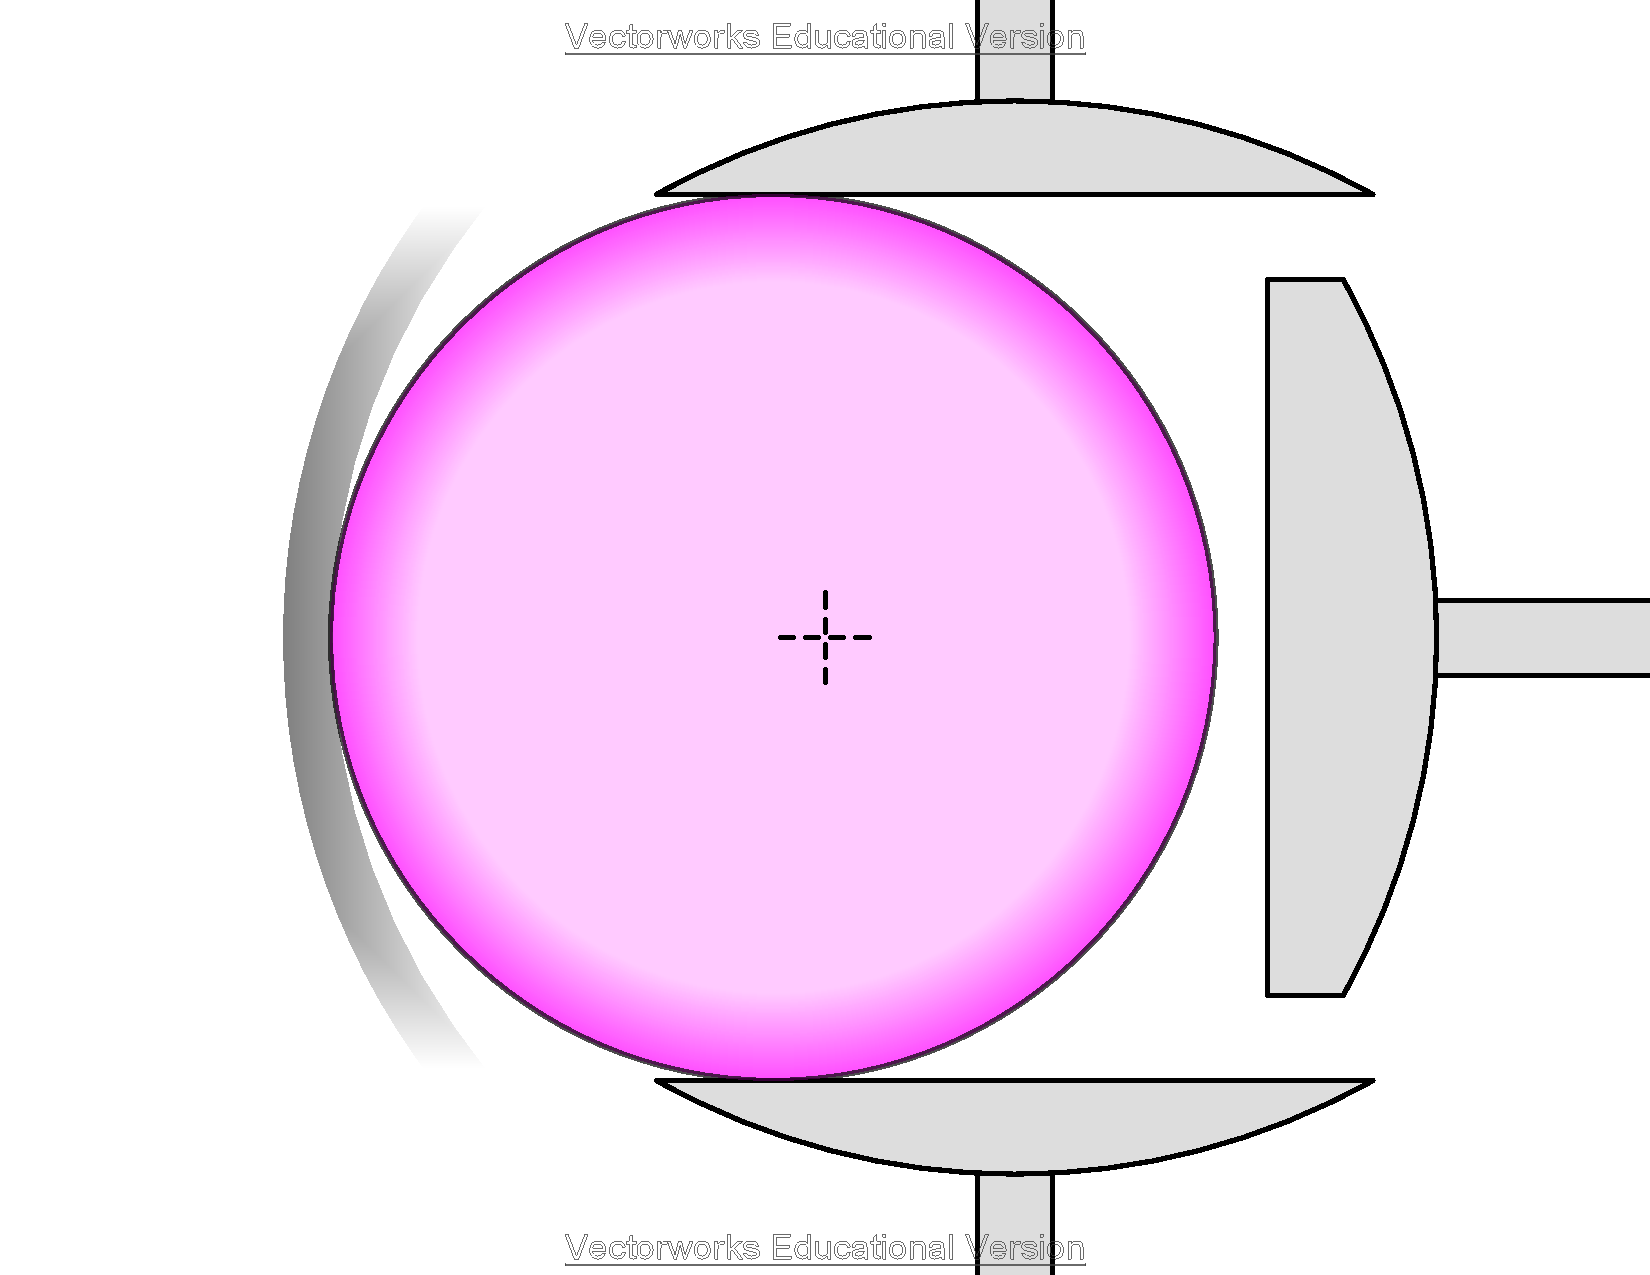
\includegraphics[width = \textwidth]{./Dissertation/figures/Poloidal_Cross_Section_v2013.pdf}\begin{flushleft}
\caption{Poloidal cross section of plasma in chamber and limiting surfaces.  Plasma is located against the inboard limiter.}
\end{flushleft}
\label{original_limiters}
\end{figure}

\subsection{Measurement of Equilibrium Parameters}
\subsubsection{Plasma Current}
The plasma current is measured by a standard rogowski coil wrapped around the insulating break at chamber \textbf{WHAT}.  Though the rogowski coil has a winding density of  \textbf{WHAT}, there can still be an effect due to fields that change rapidly on spatial scales of order the winding spacing.  Though there is little effect from the pre-existing equilibrium field coils, the shaping coil, due to it's close-set, contra-directed current bundles, has just such a field.  A minor effect, equivalent to a spurious signal equivalent to $\sim 100$A of plasma current is observed in the raw signal.  The removal of this signal is highly sucessful, and will be discussed in detail later in this thesis.
\subsubsection{Major Radius}
The radial location of the plasma is determined using a Rogowski coil with a winding density that varies as cos($\Theta$).  Due to the non-uniform winding density and the low nominal signal, this coil is much more susceptible to spurious signals due to the sharply spatially varying shaping coil field.  False displacements of $\sim 0.5cm$ have been observed when the shaping coil is energized.  This effect is removed in post processing in the same way the effects on the plasma current rogowski.
\section{Plasma Control}
\subsection{Passive Shells}
\subsection{Active Control Coils}
\section{Mode Detection}
HBT-EP is instrumented with three arrays of sensors, which measure Mirnov ($\dot{B}$) oscillations in both the poloidal and radial magnetic fields.  There are five complete toroidal arrays, at different poloidal locations, and two complete poloidal arrays, toroidally $180^{\circ}$ from each other.

\begin{figure}
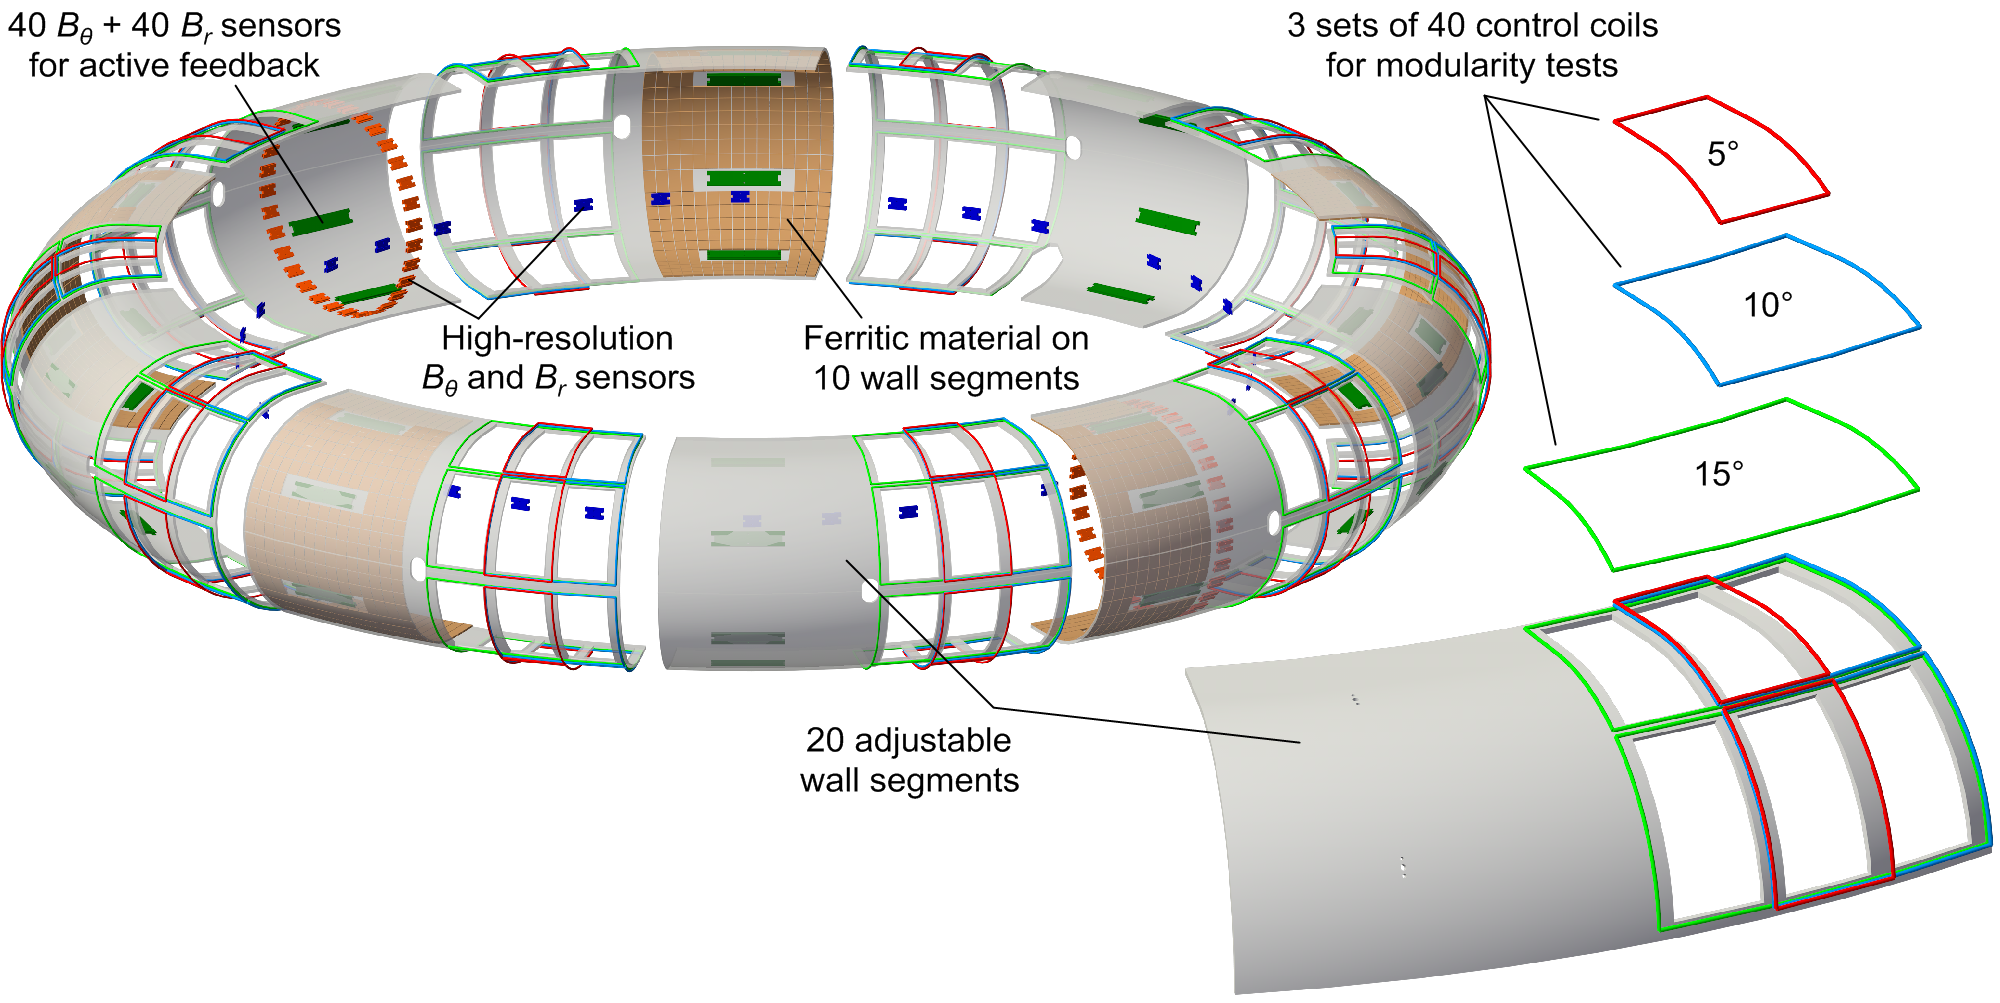
\includegraphics[width = \textwidth]{./Dissertation/figures/Plasma_with_sensors_FWall_concept_WithCCview.png}\begin{flushleft}
\caption{Schematic of HBT-EP with sensor arrays indicated.  Poloidal arrays are in red, toroidal array is in blue, and feedback arrays are in green.}
\end{flushleft}
\label{PA_sensors}
\end{figure}

As the sensors are in-vessel, and mounted close to the plasma they are shielded by 0.008 inch thick 316 stainless steel shimstock.  The equation for the rollover frequency - the frequency above which a fluctuating magnetic field is attenuated by a factor of 1/e or more as it passes through the conductor - is found by the following equation:

\begin{equation}
\omega = \frac{1}{\delta^2 \sqrt{(\frac{\mu}{2\rho})^2-\frac{\mu\epsilon}{\delta^2}}}
\end{equation}
Given the thickness and resistivity of the shimstock we can simplify this equation to:

\begin{equation}
\omega = \frac{1}{\frac{\delta^2\mu}{2\rho}}
\end{equation}

And find a rollover frequency of ~30MHz.  The MHD modes that are studied in this  paper have a frequency of 5-10kHz, so the signal will have minimal attenuation at the sensors due to eddies in the shielding.

\subsection{The Poloidal Arrays}
Chambers 3 and 8 each have a poloidal array, consisting of 32 HD sensor forms.  Each shell has 9 sensors mounted directly to the shell, with the inboard side covered by 14 sensors mounted on a thin stainless steel rib.  Every other sensor has windings to measure radial field fluctuations while all sensors are wound to measure poloidal field fluctuations.

\subsection{The Toroidal Array}
The toroidal array consists of 30 sensors, in 10 groups of 3.  Within each group, the sensors are separated by $9^{\circ}$, and each group is separated by $36^{\circ}$.  The central sensor in each group of three is wound to measure radial fields, and all sensors measure poloidal fields.  

\subsection{The Feedback Arrays}
There are four toroidal arrays of ten sensors, each wound to measure poloidal and radial fields.  The arrays are mounted two to a shell, at different \textbf{WHAT ANGLES} angles
\section{Signal Digitization}
The $\dot{B}$ sensors' measurements are integrated in both hardware, using an RC integrator, and software, using a simple trapezoidal integration technique to provide a signal representative of the actual poloidal and radial fields as a function of time.  